\documentclass{article}
\usepackage[UTF8]{ctex} 
\usepackage{amsmath}
\usepackage{bm}
\usepackage{amssymb}
\usepackage{geometry}
\usepackage{graphicx}
\usepackage{listings}
\usepackage{tikz}
\usetikzlibrary{arrows.meta, positioning, shapes.geometric}
\usetikzlibrary{decorations.pathreplacing, fit}
\geometry{a4paper, margin=1.5cm}

\title{树}
\author{Tan Yiqing}
\date{\today}

\begin{document}
\maketitle
    
    \begin{figure}[h]
        \centering
        \includegraphics[width=0.8\textwidth]{"D:/program/data_construction/firefly/v2-3e05fcc5b3b513bdf823b1d65d6cd4c7_r.jpg"}
    \end{figure}

\section{树的基本概念}
\subsection{树的定义}
\indent 树是一个 n 个结点的有限集合。当 n = 0 时,称为空树。
如果非空,则满足以下条件:
\begin{itemize}
    \item 有且仅有一个特殊的结点称为根结点。
    \item 当n$>$1时,其余结点可分为m(m$\geq$1)个互不相交的有限集合T1,T2,...,Tm,其中每个集合本身又是一棵树,称为根结点的子树。
\end{itemize}
这意味着树的很多算法是使用递归实现的。


\subsection{树的术语}
\begin{itemize}
    \item 结点的度:结点所拥有的子树的个数。
    \item 树的度:树中各结点度的最大值。
    \item 叶结点:度为 0 的结点,也称为终端结点。
    \item 分支结点:度不为 0 的结点,也称为非终端结点。
    \item 结点的层次:根结点的层数为 1;对其他结点,若某结点在第 k 层,那么其孩子结点在第 k + 1 层。
    \item 树的高度:树中所有结点的最大层次。
    \item 层序编号:从上到下、从左到右对树中结点进行编号。
    \item 孩子、双亲:一个结点拥有的子树,其根结点称为这个结点的孩子;而同时该结点亦为其孩子的双亲(比如 B 是 A 的孩子;A 是 B 的双亲)
    \item 祖先、子孙:从根结点到某一结点 p 的路径上所有结点(不包括结点 p)都是结点 p 的祖先,而结点 p 是这些结点的后代。
    \item 兄弟:具有同一个双亲的结点称为兄弟。
    \item 有序树、无序树:如果树中每个结点的子树有一个从左到右的次序,则称该树为有序树,否则称为无序树。
    \item 森林:m(m$\geq$0)棵互不相交的树的集合称为森林。当m=0时,称为空森林;当m=1时,森林中只有一棵树,此时森林退化为树。
    \item 路径:从结点p到结点q所经过的结点及边的序列称为从p到q的路径。
    \item 路径长度:路径上边的数目。
\end{itemize}

\subsection{与线性结构的区别}
\begin{itemize}
    \item 线性结构中每个结点最多只有一个前驱和一个后继,而树中每个结点可以有多个孩子。
    \item 线性结构中只有一个结点没有前驱(头结点),而树中只有一个结点没有双亲(根结点)。
    \item 线性结构中只有一个结点没有后继(尾结点),而树中可以有多个叶结点。
\end{itemize}

\subsection{树的遍历}
\indent 遍历树是指按某种次序访问树中所有结点且每个结点只访问一次。常用的遍历方法有前序遍历、后序遍历和层次遍历。
假设树为:
\begin{figure}[h]
    \centering
    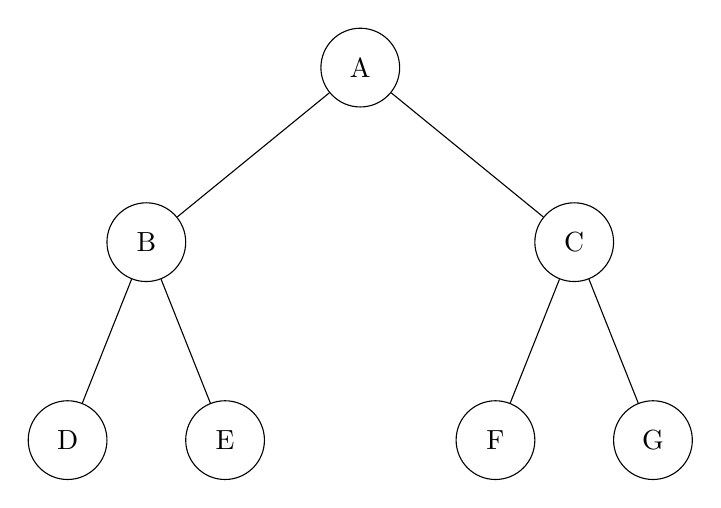
\begin{tikzpicture}[node distance=1.5cm and 2cm, every node/.style={circle, draw, minimum size=1cm}]
        \node (A) {A};
        \node (B) [below left=of A] {B};
        \node (C) [below right=of A] {C};
        \node (D) [below=1.5cm of B, xshift=-1cm] {D};
        \node (E) [below=1.5cm of B, xshift=1cm] {E};
        \node (F) [below=1.5cm of C, xshift=-1cm] {F};
        \node (G) [below=1.5cm of C, xshift=1cm] {G};
        
        \draw (A) -- (B);
        \draw (A) -- (C);
        \draw (B) -- (D);
        \draw (B) -- (E);
        \draw (C) -- (F);
        \draw (C) -- (G);
    \end{tikzpicture}
    \caption{树的示例}
\end{figure}

\subsubsection{前序遍历}
\indent 若空树,则遍历完成。先访问根结点,然后依次从左到右遍历各个子树。即:A-B-D-E-C-F-G。
\subsubsection{后序遍历}
\indent 若空树,则遍历完成。先依次从左到右遍历各个子树,然后访问根结点。即:D-E-B-F-G-C-A。
\subsubsection{层次遍历}
\indent 若空树,则遍历完成。先访问根结点,然后依次从上到下、从左到右遍历各个子树。该方法没有使用树本身的结构。即:A-B-C-D-E-F-G。

\subsubsection{确定树的唯一性}
知道前序和后序,可以唯一确定树。方法为:
\begin{itemize}
    \item 1. 前序遍历的第一个结点一定是根结点。
    \item 2. 在后序遍历中找到根结点的位置,根结点左边的部分对应左子树,右边的部分对应右子树(如果有多棵子树,则依次划分)。
    \item 3. 在前序和后序序列中递归地对应每一棵子树,重复上述过程,直到所有结点都被确定。
    \item 4. 由于树的结构是有序的(即每个结点的孩子有顺序为从左往右,且不分左右),所以可以唯一还原整棵树。
\end{itemize}

\textbf{举例:}

已知前序遍历为:A B D E C F G

已知后序遍历为:D E B F G C A

\begin{enumerate}
    \item 根结点为A(前序第一个,后序最后一个)。
    \item 在后序中,D E B 是A的左子树,F G C 是A的右子树。
    \item 前序中,A后面的B D E对应左子树,C F G对应右子树。
    \item 递归处理左子树和右子树,依次确定所有结点的父子关系。
\end{enumerate}

\section{树的实现}
\subsection{双亲表示法}
\indent 双亲表示法使用一个一维数组来存储树中的结点。每个结点包含两个信息:结点的值和其双亲结点在数组中的下标。根结点的双亲下标通常设为-1或其他特殊值表示没有双亲。
\subsection{孩子表示法}
\indent 孩子表示法使用一个一维数组来存储树中的结点,每个结点包含两个信息:结点的值和其第一个孩子结点在数组中的下标。根结点的孩子下标通常设为-1或其他特殊值表示没有孩子。每个结点的兄弟结点通过下标关系来表示。
\subsection{孩子兄弟表示法}
\indent 孩子兄弟表示法使用一个一维数组来存储树中的结点。每个结点包含三个信息:结点的值、第一个孩子结点在数组中的下标和下一个兄弟结点在数组中的下标。根结点的孩子和兄弟下标通常设为-1或其他特殊值表示没有孩子或兄弟。

\section{二叉树}
\subsection{定义}
\indent 二叉树是 n 个结点的有限集合。当集合为空时,称为空二叉树。非空时,则有一个根结点以及两颗互不相交的二叉树构成(分别为左子树、右子树)。
\begin{center}
    \LARGE \pmb{二叉树不是树!!!}\\
    \LARGE \pmb{核心区别:二叉树区分左右!!!可以有右孩子没有左孩子。}
\end{center}
\subsection{术语}
\begin{itemize}
    \item 满二叉树:一棵深度为k的二叉树,若其所有叶结点都在第k层,且每个非叶结点都有两个孩子,则称该二叉树为满二叉树。
    \item 完全二叉树:设二叉树的深度为k,除第k层外,其余各层上的结点数都达到最大值,第k层所有结点都连续集中在最左边,则称该二叉树为完全二叉树。
    \item 二叉搜索树:若它是一棵空树,或它的左子树上所有结点的值均小于根结点的值,且它的右子树上所有结点的值均大于根结点的值,并且它的左、右子树也分别为二叉搜索树,则称该二叉树为二叉搜索树。
    \item 平衡二叉树:一棵空树,或它的左、右子树都是平衡二叉树,且左、右子树的高度之差的绝对值不超过1,则称该二叉树为平衡二叉树。
    \item 斜树:每个结点只有一个左或右孩子的二叉树称为斜树。
\end{itemize}

\noindent 完全二叉树的判别(算法流程):
\begin{itemize}
    \item 只有右孩子没有左孩子,不是完全二叉树
	\item 出现了只有左孩子而没有右孩子,or没有孩子,则后面只能出现叶子结点
\end{itemize}

\subsection{性质}
\begin{itemize}
    \item 在二叉树的第i层上至多有2$^{i-1}$个结点(i$\geq$1)。
    \item 深度为k的二叉树至多有2$^k$-1个结点(k$\geq$1)。
    \item 对于任何一棵二叉树T,设其叶结点数为n0,度为2的结点数为n2,则有n0=n2+1。
\end{itemize}

\subsection{完全二叉树特性}
\indent 设完全二叉树的深度为k,结点总数为n,则有:
\[2^{k-1} \leq n < 2^k\]
高度至少为$\lfloor \log_2(n) \rfloor + 1$,至多为n。
\indent 设完全二叉树的结点按层序从上到下、从左到右编号,则对于任意结点i:
\begin{itemize}
    \item 若i=1,则结点i为根结点,无双亲。
    \item 若i$>$1,则结点i的双亲为$\left\lfloor \frac{i}{2} \right\rfloor$。
    \item 若2i$\leq$ n,则结点i的左孩子为2i。
    \item 若2i+1$\leq$ n,则结点i的右孩子为2i+1。
\end{itemize}
\indent 完全二叉树可以用顺序结构实现。

\subsection{二叉树的遍历}
二叉树的遍历包括前序遍历、中序遍历、后序遍历和层次遍历。假设二叉树为:
\begin{figure}[h]
    \centering
    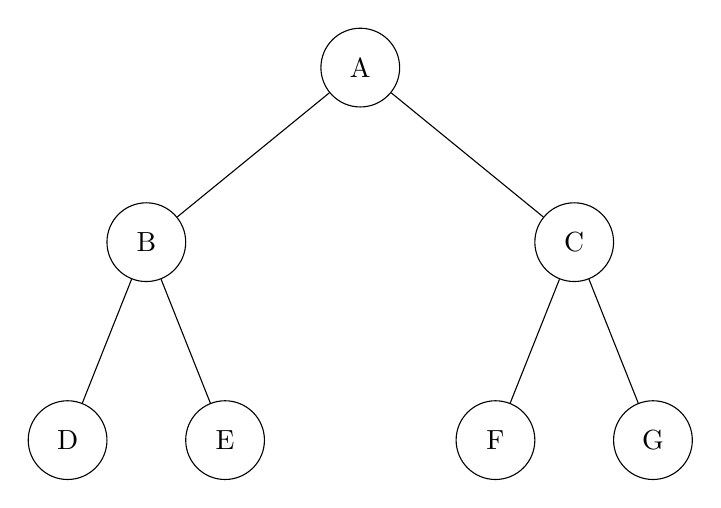
\begin{tikzpicture}[node distance=1.5cm and 2cm, every node/.style={circle, draw, minimum size=1cm}]
        \node (A) {A};
        \node (B) [below left=of A] {B};
        \node (C) [below right=of A] {C};
        \node (D) [below=1.5cm of B, xshift=-1cm] {D};
        \node (E) [below=1.5cm of B, xshift=1cm] {E};
        \node (F) [below=1.5cm of C, xshift=-1cm] {F};
        \node (G) [below=1.5cm of C, xshift=1cm] {G};
        
        \draw (A) -- (B);
        \draw (A) -- (C);
        \draw (B) -- (D);
        \draw (B) -- (E);
        \draw (C) -- (F);
        \draw (C) -- (G);
    \end{tikzpicture}
    \caption{二叉树的示例}
\end{figure}
\subsubsection{前序遍历}
\indent 前序遍历的顺序为:根结点 - 左子树 - 右子树。如:A-B-D-E-C-F-G。
\subsubsection{中序遍历}
\indent 中序遍历的顺序为:左子树 - 根结点 - 右子树。如:D-B-E-A-F-C-G。
\subsubsection{后序遍历}
\indent 后序遍历的顺序为:左子树 - 右子树 - 根结点。如:D-E-B-F-G-C-A。
\subsubsection{层次遍历}
\indent 层次遍历的顺序为:从上到下、从左到右。如:A-B-C-D-E-F-G。


\subsubsection{确定\pmb{二叉树}的唯一性}
知道前序和中序,可以唯一确定二叉树。方法为:
\begin{itemize}
    \item 1. 前序遍历的第一个结点一定是根结点。
    \item 2. 在中序遍历中找到根结点的位置,根结点左边的部分对应左子树,右边的部分对应右子树。
    \item 3. 在前序和中序序列中递归地对应每一棵子树,重复上述过程,直到所有结点都被确定。
    \item 4. 由于二叉树的结构是有序的(即每个结点的左、右孩子有顺序),所以可以唯一还原整棵二叉树。
\end{itemize}
\textbf{举例:}
已知前序遍历为:A B D E C F G
已知中序遍历为:D B E A F C G
\begin{enumerate}
    \item 根结点为A(前序第一个,后序最后一个)。
    \item 在中序中,D B E 是A的左子树,F C G 是A的右子树。
    \item 前序中,A后面的B D E对应左子树,C F G对应右子树。
    \item 递归处理左子树和右子树,依次确定所有结点的父子关系。
    \item 最终还原出唯一的二叉树结构。
\end{enumerate}

\indent 后序加中序也可以唯一确定二叉树。方法为:
\begin{itemize}
    \item 1. 后序遍历的最后一个结点一定是根结点。
    \item 2. 在中序遍历中找到根结点的位置,根结点左边的部分对应左子树,右边的部分对应右子树。
    \item 3. 在后序和中序序列中递归地对应每一棵子树,重复上述过程,直到所有结点都被确定。
    \item 4. 由于二叉树的结构是有序的(即每个结点的左、右孩子有顺序),所以可以唯一还原整棵二叉树。
\end{itemize}
\textbf{举例:}
已知后序遍历为:D E B F G C A
已知中序遍历为:D B E A F C G
\begin{enumerate}
    \item 根结点为A(后序最后一个,中序第一个)。
    \item 在中序中,D B E 是A的左子树,F C G 是A的右子树。
    \item 后序中,D E B对应左子树,F G C对应右子树。
    \item 递归处理左子树和右子树,依次确定所有结点的父子关系。
    \item 最终还原出唯一的二叉树结构。
\end{enumerate}
\indent 方法要点:找重复出现但顺序不同的部分来区分左、右、根。\\
\indent 但是\pmb{前序和后序}无法确定唯一二叉树,根本原因是二叉树区分左右。

\begin{center}
    \fbox{
        \begin{minipage}{0.9\textwidth}
            \textbf{Proposition:} 已知前序和中序遍历,可以唯一确定二叉树。
        \end{minipage}
    }
\end{center}

\begin{center}
    \fbox{
        \begin{minipage}{0.9\textwidth}
            \textbf{Proof}:当结点是0或1时,结论明显。\\
            \indent 假设对少于$n$个结点的二叉树结论成立,现考虑$n$个结点的二叉树。\\
            \indent 设前序遍历序列为 $P_{1}, P_{2}, \ldots, P_{n}$,中序遍历序列为 $M_{1}, M_{2}, \ldots, M_{n}$。\\
            \indent 根据前序定义,$P_{1}$ 为根结点。那么存在 $1 \leq i \leq n$,使得 $M_{i} = P_{1}$。\\
            \indent 按照中序的定义,$M_{1}, M_{2}, \ldots, M_{i-1}$ 为左子树的中序遍历序列,$M_{i+1}, M_{i+2}, \ldots, M_{n}$ 为右子树的中序遍历序列。\\
            \indent 又根据前序的定义,$P_{2}, P_{3}, \ldots, P_{i}$ 为左子树的前序遍历序列,$P_{i+1}, P_{i+2}, \ldots, P_{n}$ 为右子树的前序遍历序列。\\
            \indent 因为$i-1<n$由归纳假设,左子树和右子树均可以唯一确定,因此整棵二叉树也可以唯一确定。\\
            \indent \textbf{Q.E.D.}
        \end{minipage}
    }
\end{center}

\subsection{存储二叉树}
\subsection{顺序储存}
\indent 一般只有完全二叉树使用顺序存储。

\subsubsection{链式存储}
\indent 每个结点由一个数据域和两个指针域组成,分别指向其左、右孩子结点的位置。

\section{二叉树遍历的递归和非递归写法}
\subsection{前序遍历}
\subsubsection{递归写法}
\indent 思路:
\begin{itemize}
    \item 若结点为空,则返回。
    \item 访问根结点。
    \item 递归遍历左子树。
    \item 递归遍历右子树。
    \item 返回。
\end{itemize}
\indent 前序遍历的递归实现如下:
\begin{lstlisting}[language=C]
void preOrder(TreeNode* root) {
    if (root == NULL) return;
    visit(root);
    preOrder(root->left);
    preOrder(root->right);
}
\end{lstlisting}

\subsubsection{非递归写法}
\indent 思路:
\begin{itemize}
    \item 使用栈来模拟递归过程。
    \item 初始化栈为空,当前结点为根结点。
    \item 当当前结点不为空或栈不为空时,重复以下步骤:
    \begin{itemize}
        \item 当当前结点不为空时,访问当前结点并输出,将其右孩子入栈,然后将当前结点更新为其左孩子。
        \item 当当前结点为空且栈不为空时,从栈中弹出一个结点,将其右孩子赋值给当前结点。
    \end{itemize}
\end{itemize}
\indent 前序遍历的非递归实现可以使用栈来模拟递归过程:
\begin{lstlisting}[language=C]
void preOrder(TreeNode* root) {
    stack<TreeNode*> s;
    TreeNode* curr = root;
    while (curr != NULL || !s.empty()) {
        while (curr != NULL) {
            visit(curr);
            s.push(curr);
            curr = curr->left;
        }
        if (!s.empty()) {
            curr = s.top();
            s.pop();
            curr = curr->right;
        }
    }
}
\end{lstlisting}

\subsection{中序遍历}
\subsubsection{递归写法}
\indent 思路:
\begin{itemize}
    \item 若结点为空,则返回。
    \item 递归遍历左子树。
    \item 访问根结点。
    \item 递归遍历右子树。
    \item 返回。
\end{itemize}
\indent 中序遍历的递归实现如下:
\begin{lstlisting}[language=C]
void inOrder(TreeNode* root) {
    if (root == NULL) return;
    inOrder(root->left);
    visit(root);
    inOrder(root->right);
}
\end{lstlisting}

\subsubsection{非递归写法}
\indent 思路:
\begin{itemize}
    \item 使用栈来模拟递归过程。
    \item 初始化栈为空,当前结点为根结点。
    \item 当当前结点不为空或栈不为空时,重复以下步骤:
    \begin{itemize}
        \item 当当前结点不为空时,将其入栈,然后将当前结点更新为其左孩子。
        \item 当当前结点为空且栈不为空时,从栈中弹出一个结点,访问该结点并输出,然后将其右孩子赋值给当前结点。
    \end{itemize}
\end{itemize}
\indent 中序遍历的非递归实现可以使用栈来模拟递归过程:
\begin{lstlisting}[language=C]
void inOrder(TreeNode* root) {
    stack<TreeNode*> s;
    TreeNode* curr = root;
    while (curr != NULL || !s.empty()) {
        while (curr != NULL) {
            s.push(curr);
            curr = curr->left;
        }
        if (!s.empty()) {
            curr = s.top();
            s.pop();
            visit(curr);
            curr = curr->right;
        }
    }
}
\end{lstlisting}

\subsection{后序遍历}
\subsubsection{递归写法}
\indent 思路:
\begin{itemize}
    \item 若结点为空,则返回。
    \item 递归遍历左子树。
    \item 递归遍历右子树。
    \item 访问根结点。
    \item 返回。
\end{itemize}
\indent 后序遍历的递归实现如下:
\begin{lstlisting}[language=C]
void postOrder(TreeNode* root) {
    if (root == NULL) return;
    postOrder(root->left);
    postOrder(root->right);
    visit(root);
}
\end{lstlisting}
\subsubsection{非递归写法}
\indent 思路:
\begin{itemize}
    \item 使用栈来模拟递归过程。(栈+指标,也就是区分是否第一次访问该结点)
    \item 初始化栈为空,当前结点为根结点,设置一个辅助指针lastVisited为NULL。
    \item 当当前结点不为空或栈不为空时,重复以下步骤:
    \begin{itemize}
        \item 当当前结点不为空时,将其入栈,然后将当前结点更新为其左孩子。
        \item 当当前结点为空且栈不为空时,查看栈顶结点:
        \begin{itemize}
            \item 如果栈顶结点的右孩子为空或已被访问过(即等于lastVisited),则访问该结点并弹出,将lastVisited更新为该结点,当前结点设为NULL。
            \item 否则,将当前结点更新为栈顶结点的右孩子。
        \end{itemize}
    \end{itemize}
\end{itemize}
\indent 后序遍历的非递归实现可以使用栈来模拟递归过程:
\begin{lstlisting}[language=C]
void postOrder(TreeNode* root) {
    stack<TreeNode*> s;
    TreeNode* curr = root;
    TreeNode* lastVisited = NULL;
    while (curr != NULL || !s.empty()) {
        while (curr != NULL) {
            s.push(curr);
            curr = curr->left;
        }
        if (!s.empty()) {
            curr = s.top();
            if (curr->right == NULL || curr->right == lastVisited) {
                visit(curr);
                s.pop();
                lastVisited = curr;
                curr = NULL;
            } else {
                curr = curr->right;
            }
        }
    }
}
\end{lstlisting}

\section{树与二叉树的等价性}
\subsection{树与二叉树之间的双射(左孩子-右兄弟表示法)}
\indent 建立方法:
\begin{itemize}
    \item 树 $\to$ 二叉树:对每个结点,将其第一个孩子作为左孩子;将每个结点的相邻兄弟用右孩子指针依次相连成右兄弟链;递归处理各子树。
    \item 二叉树 $\to$ 树:对每个结点,其左孩子是第一个孩子;从该孩子起沿右孩子指针依次枚举兄弟,作为当前结点的其余孩子;递归处理。
\end{itemize}
\indent 两步互为逆映射,故在有序根树与左孩子-右兄弟二叉树之间建立双射。

\begin{figure}[h]
    \centering
    \begin{tikzpicture}[every node/.style={circle, draw, minimum size=7mm, font=\small}]
        %---------------- Left: Tree ----------------%
        \node[draw=none, circle=none, font=\bfseries] at (-5,3) {树};
        \node (A) at (-5,2) {A};
        \node (B) at (-6,0) {B};
        \node (C) at (-5,0) {C};
        \node (D) at (-4,0) {D};
        \node (E) at (-6.6,-1.8) {E};
        \node (F) at (-5.4,-1.8) {F};
        \node (G) at (-4,-1.8) {G};
        \draw[thick] (A) -- (B) (A) -- (C) (A) -- (D);
        \draw[thick] (B) -- (E) (B) -- (F);
        \draw[thick] (D) -- (G);
        \node[draw=gray, dashed, fit=(A)(B)(C)(D)(E)(F)(G), inner sep=6pt] {};

        %---------------- Right: LC-RS Binary Tree ----------------%
        \node[draw=none, circle=none, font=\bfseries] at (3.8,3) {LC-RS 二叉树};
        \node (A2) at (2,2) {A};
        \node (B2) at (2,0) {B};
        \node (C2) at (3.6,0) {C};
        \node (D2) at (5.2,0) {D};
        \node (E2) at (2,-2) {E};
        \node (F2) at (3.2,-2) {F};
        \node (G2) at (5.2,-2) {G};
        % 左孩子边(实线)
        \draw[thick] (A2) -- (B2);
        \draw[thick] (B2) -- (E2);
        \draw[thick] (D2) -- (G2);
        % 右兄弟边(虚线箭头)
        \draw[dashed, -{Latex}, thick] (B2) -- (C2);
        \draw[dashed, -{Latex}, thick] (C2) -- (D2);
        \draw[dashed, -{Latex}, thick] (E2) -- (F2);
        \node[draw=gray, dashed, fit=(A2)(B2)(C2)(D2)(E2)(F2)(G2), inner sep=6pt] {};

        %---------------- Legend ----------------%
        \node[draw=none, circle=none, font=\small] at (3.8,-3) {图例:};
        \draw[thick] (2.2,-3.4) -- (2.9,-3.4);
        \node[draw=none, circle=none, font=\small] at (3.8,-3.4) {左孩子边};
        \draw[dashed, -{Latex}, thick] (2.2,-3.9) -- (2.9,-3.9);
        \node[draw=none, circle=none, font=\small] at (4.0,-3.9) {右兄弟边};
    \end{tikzpicture}
    \caption{树与二叉树(左孩子-右兄弟)的双射示意}
\end{figure}
\subsection{遍历对应下的结点访问顺序}
\indent 设树用“左孩子-右兄弟”法转为对应二叉树,则有:
\begin{itemize}
    \item 树的前序遍历 顺序 = 对应二叉树的前序遍历 顺序。
    \item 树的后序遍历 顺序 = 对应二叉树的中序遍历 顺序。
\end{itemize}

\noindent 以上图示中的示例(A 根,孩子依次为 B,C;B 的孩子为 D,E;C 的孩子为 F,G):
\begin{itemize}
    \item 树的前序:A, B, D, E, C, F, G
    \item 二叉树的前序:A, B, D, E, C, F, G
    \item 树的后序:D, E, B, F, G, C, A
    \item 二叉树的中序:D, E, B, F, G, C, A
\end{itemize}

\noindent 注:层次遍历在该对应下不保持不变;上述“二叉树”均指左孩子-右兄弟表示得到的二叉树。

\section{应用}
\subsection{哈夫曼树与编码}
\indent 假设有一个字符串,其中只有字母A,B,C,一般情况下我们用ASCII码,每个字符用了8个bit的空间,如何少用空间呢? \\
\indent 其实这里就只是三个不同的字符,所以每个用2个bit就行,如下表所示:

\begin{center}
\begin{tabular}{|c|c|}
\hline
字符 & 编码 \\
\hline
A & 00 \\
B & 01 \\
C & 10 \\
\hline
\end{tabular}
\end{center}

\indent 这个过程就叫做编码,如果知道每个字符出现的频率,我们可能做的更好。\\
\subsubsection{编码:}
数学上,一个编码的码字集合C,原本的字符集M,那么编码就是M到C的一个单射。计算机上,码字集合一般为0,1的数组川。\\
\subsubsection{前缀编码:}
所有码字都不是其他码字的前缀。它的优点是对给出的已编码串,可以唯一解出原文。\\
\subsubsection{哈夫曼树}
\indent 问题:给定一组字符与每个字符在文章中的使用次数,设计一种编码方案,使得编码后的文章长度最短。符合问题要求的编码就叫\pmb{哈夫曼编码},用于生成哈夫曼编码的树就叫\pmb{哈夫曼树}。\\
\indent 其实每一个使用0、1编码的过程都可以看成是一棵二叉树,左子树代表0,右子树代表1。
那么问题转化为寻找符合上述条件的最小带权长度(weight path length, WPL)的二叉树。\\
\indent 哈夫曼树的构造算法如下:
\begin{itemize}
    \item 1. 对每个字符做一个结点,权重为使用频率,进而得到一个森林。
    \item 2. 若森林里的树的数目多于一棵时:
    \item     2a. 选出权(如为单结点)或叶子权值总和(若为已合并过的树)最小的两棵树。
    \item     2b. 构造一棵新树,其左、右孩子为上步选择的两棵树。
    \item     2c. 删掉那两颗树,并把新树加到森林中去。
    \item 3. 剩下的这棵树即为符合要求编码的对应哈夫曼树。(Rmk:答案不一定唯一,但WPL唯一)
\end{itemize}

\indent 哈夫曼算法的贪心选择性质:
\begin{center}
    \fbox{
        \begin{minipage}{0.9\textwidth}
            设$C$为字符集,$x$和$y$为其中两个频率最小的字符。则存在一棵最优哈夫曼树,其中$x$和$y$是最深的两个叶子结点。
        \end{minipage}
    }
\end{center}
\begin{center}
    \fbox{
        \begin{minipage}{0.9\textwidth}
            \textbf{Proof}:设$T$为一棵最优哈夫曼树,$a$和$b$为$T$中最深的两个叶子结点。\\
            \indent 交换$x$与$a$的位置,得到新树$T'$。则有:
            \begin{align*}
                WPL(T') - WPL(T) &= f(x)d_{T'}(x) + f(a)d_{T'}(a) - f(x)d_{T}(x) - f(a)d_{T}(a) \\
                &= (f(a) - f(x))(d_{T}(x) - d_{T}(a)) \\
                &\leq 0
            \end{align*}
            \indent 同理,交换$y$与$b$的位置,得到新树$T''$,则有:
            \begin{align*}
                WPL(T'') - WPL(T') &= f(y)d_{T''}(y) + f(b)d_{T''}(b) - f(y)d_{T'}(y) - f(b)d_{T'}(b) \\
                &= (f(b) - f(y))(d_{T'}(y) - d_{T'}(b)) \\
                &\leq 0
            \end{align*}
            \indent 因此,$WPL(T'') \leq WPL(T') \leq WPL(T)$,且由于$T$为最优哈夫曼树,故$WPL(T'') = WPL(T)$。\\
            \indent 由此可见,存在一棵最优哈夫曼树,其中$x$和$y$是最深的两个叶子结点。\\
            \indent \textbf{Q.E.D.}
        \end{minipage}
    }
\end{center}

\end{document}